\chapter{Giới thiệu}
\label{Chapter1}
\setcounter{secnumdepth}{5}

\section{Bối cảnh chung}
    Trong thập kỷ qua, các mạng học sâu ứng dụng trong lĩnh vực Thị giác Máy tính đã đạt được nhiều thành tựu quan trọng trong các tác vụ như phân loại ảnh, phát hiện đối tượng và phân đoạn ảnh. Các kiến trúc như mạng nơ-ron tích chập (Convolutional Neural Networks -- CNNs) và Vision Transformer đã giúp mô hình học được các đặc trưng trực quan phức tạp từ dữ liệu hình ảnh, từ đó cải thiện đáng kể độ chính xác so với các phương pháp xử lý ảnh truyền thống. Tuy nhiên, phần lớn các mô hình này vẫn hoạt động trong bối cảnh \textit{Closed-vocabulary}, nghĩa là chúng chỉ có thể nhận diện hoặc phân đoạn các lớp đối tượng đã được định nghĩa sẵn trong tập dữ liệu huấn luyện.

    Cách tiếp cận \textit{Closed-vocabulary} tạo ra một giới hạn lớn về khả năng tổng quát hóa. Khi mô hình được triển khai trên các miền dữ liệu mới, các lớp đối tượng mới, hoặc các điều kiện thu nhận ảnh khác biệt so với dữ liệu huấn luyện, hiệu suất thường suy giảm đáng kể. Nguyên nhân là mô hình học mối quan hệ chặt chẽ giữa hình ảnh và tập nhãn cố định, nhưng không có cơ chế linh hoạt để hiểu các khái niệm mới ngoài tập nhãn đó. Điều này đặc biệt bất lợi trong các bài toán thực tế, nơi dữ liệu luôn đa dạng, phân bố thay đổi theo thời gian, và yêu cầu nhận diện có thể thay đổi tùy theo ngữ cảnh sử dụng.

    Sự xuất hiện của các mô hình nền tảng (Foundation Models) như CLIP và SAM đã thúc đẩy sự chuyển dịch từ các hệ thống phân đoạn khép kín sang các hệ thống có khả năng tương tác và mở rộng hơn. CLIP cho thấy hiệu quả của việc học biểu diễn chung giữa hình ảnh và ngôn ngữ tự nhiên, trong khi SAM chứng minh khả năng phân đoạn linh hoạt thông qua các dạng prompt trực quan như điểm, hộp bao hoặc mặt nạ gợi ý. Những mô hình này mở ra hướng tiếp cận \textit{Open-vocabulary Segmentation}, trong đó mô hình không chỉ phụ thuộc vào tập nhãn cố định, mà có thể sử dụng thông tin mô tả bổ sung để xác định vùng cần phân đoạn.

    Trong bối cảnh này, prompt đóng vai trò như một kênh giao tiếp giữa người dùng và mô hình. Prompt có thể tồn tại dưới nhiều dạng khác nhau, chẳng hạn như điểm ảnh, hộp bao, mặt nạ thô hoặc mô tả bằng ngôn ngữ tự nhiên. Đối với phân đoạn dựa trên văn bản, câu nhắc văn bản giúp người dùng mô tả trực tiếp đối tượng, cơ quan hoặc vùng tổn thương cần quan tâm. Nhờ đó, mô hình có khả năng khai thác thêm thông tin ngữ nghĩa thay vì chỉ dựa trên tín hiệu thị giác thuần túy.

    Tuy nhiên, đối với nhiều lĩnh vực chuyên biệt, đặc biệt là trong y khoa, việc ứng dụng các mô hình học sâu vẫn bị giới hạn bởi sự thiếu hụt các tập dữ liệu được dán nhãn chất lượng cao \cite{li_lvit_2023}. Dữ liệu y khoa thường có chi phí thu thập và gán nhãn rất lớn, bởi quá trình chú thích cần được thực hiện hoặc kiểm chứng bởi bác sĩ và chuyên gia có kinh nghiệm. Ngoài ra, ranh giới của các cấu trúc giải phẫu hoặc tổn thương bệnh lý thường không rõ ràng, có sự khác biệt giữa các chuyên gia, và phụ thuộc mạnh vào từng phương thức hình ảnh như CT, MRI, siêu âm hoặc nội soi.
    
    Chính vì vậy, bên cạnh dữ liệu hình ảnh, các mô hình hiện đại có xu hướng phát triển các cơ chế học dựa trên câu nhắc (\textit{Prompting}) nhằm tận dụng tri thức đa phương thức. Thay vì yêu cầu một lượng lớn nhãn pixel chính xác cho mọi bệnh lý và mọi cơ quan, mô hình có thể khai thác thông tin bổ sung từ văn bản lâm sàng, báo cáo chẩn đoán hoặc mô tả chuyên môn. Cách tiếp cận này giúp thu hẹp khoảng cách giữa dữ liệu hình ảnh và tri thức y khoa, đồng thời hỗ trợ mô hình tập trung vào vùng có ý nghĩa lâm sàng.

    Một số mô hình tiêu biểu cho xu hướng này gồm:
        \begin{itemize}
            \item \textbf{MedSAM:} Kế thừa khả năng phân đoạn linh hoạt của SAM và sử dụng \textit{câu nhắc trực quan} như điểm hoặc hộp bao để hướng dẫn mô hình tập trung vào vùng giải phẫu hoặc tổn thương cần phân đoạn.
            \item \textbf{LViT:} Tích hợp \textit{câu nhắc văn bản} vào quá trình học biểu diễn, giúp đưa kiến thức bệnh lý và thông tin mô tả lâm sàng vào mô hình phân đoạn, từ đó cải thiện hiệu suất trong điều kiện dữ liệu nhãn còn hạn chế.
        \end{itemize}

    Sự hiệu quả của các kiến trúc kết hợp Prompting bắt nguồn từ khả năng thiết lập một không gian biểu diễn chung giữa thị giác và ngôn ngữ thông qua cơ chế căn chỉnh đa phương thức. Trong không gian này, đặc trưng hình ảnh không còn được xử lý một cách độc lập, mà được điều hướng bởi các khái niệm ngữ nghĩa được cung cấp từ prompt. Nhờ đó, mô hình có thể hình thành một bộ lọc ngữ nghĩa mạnh mẽ, giúp giảm ảnh hưởng của các vùng nhiễu, loại bỏ các cấu trúc không liên quan và tập trung vào những đặc điểm phù hợp với mô tả đầu vào.

    Đối với ảnh y khoa, vai trò của ngôn ngữ càng trở nên quan trọng vì nhiều tổn thương không thể được xác định chỉ bằng tên lớp đơn giản. Thay vì chỉ biết đây là ``khối u'', văn bản có thể cung cấp thêm các đặc điểm hình thái chuyên sâu như \textit{``bờ không đều'', ``mật độ thấp'', ``thâm nhiễm xung quanh''} hoặc vị trí tương quan với các cấu trúc giải phẫu lân cận. Những mô tả này giúp mô hình hiểu rõ hơn ngữ cảnh bệnh lý, từ đó đưa ra mặt nạ phân đoạn hợp lý hơn về mặt y khoa.

    Do đó, phân đoạn ảnh dựa trên prompt, đặc biệt là prompt văn bản, là một hướng nghiên cứu có ý nghĩa trong việc xây dựng các hệ thống phân đoạn linh hoạt, có khả năng thích ứng với dữ liệu mới và phù hợp hơn với quy trình làm việc thực tế của chuyên gia. Đây cũng là nền tảng quan trọng để phát triển các mô hình hỗ trợ chẩn đoán có tính tương tác, tận dụng đồng thời thông tin thị giác và tri thức chuyên ngành được biểu diễn bằng ngôn ngữ tự nhiên.
\section{Động lực nghiên cứu}
\subsection{Ý nghĩa khoa học}
    Sự phát triển của trí tuệ nhân tạo và thị giác máy tính trong nhiều lĩnh vực đã chứng minh vai trò quan trọng của phân đoạn ảnh tự động. Khác với bài toán phân loại ảnh chỉ đưa ra nhãn tổng quát cho toàn bộ ảnh, phân đoạn ảnh yêu cầu mô hình xác định chính xác vùng không gian tương ứng với từng đối tượng hoặc từng cấu trúc quan tâm. Vì vậy, phân đoạn ảnh đóng vai trò nền tảng trong nhiều hệ thống phân tích hình ảnh chuyên sâu, đặc biệt là các hệ thống cần định lượng hình dạng, kích thước, vị trí hoặc mức độ lan rộng của đối tượng như hệ thống xe tự hành, hệ thống giám sát nông nghiệp, hệ thống chỉnh sửa ảnh/video, hệ thống kiểm tra chất lượng sản phẩm, hệ thống phân tích ảnh y tế,...

    Tuy nhiên, hiệu quả của các mô hình phân đoạn học sâu phụ thuộc rất lớn vào chất lượng và quy mô của dữ liệu được gán nhãn ở mức pixel. Việc tạo ra các nhãn chuẩn này không chỉ tiêu tốn nhiều chi phí và thời gian, mà còn đòi hỏi sự tham gia trực tiếp của các chuyên gia có kiến thức chuyên môn. Trong y khoa, yêu cầu này càng trở nên nghiêm ngặt hơn vì ranh giới của cơ quan, mô bệnh hoặc tổn thương thường khó xác định, dễ bị ảnh hưởng bởi nhiễu ảnh, độ tương phản thấp và sự khác biệt giữa các thiết bị chụp. Do đó, việc xây dựng các bộ dữ liệu lớn, đa dạng và được chú thích chính xác vẫn là một thách thức lớn.

    Về mặt khoa học, hạn chế về dữ liệu nhãn đặt ra nhu cầu nghiên cứu các phương pháp có khả năng học hiệu quả hơn từ ít dữ liệu hơn, đồng thời tận dụng được các nguồn tri thức bổ sung ngoài nhãn pixel truyền thống. Các mô hình dựa trên prompt, đặc biệt là prompt văn bản, cung cấp một hướng tiếp cận tiềm năng cho vấn đề này. Thay vì chỉ học từ cặp ảnh-mặt nạ, mô hình có thể khai thác thêm mô tả ngôn ngữ về đặc điểm hình thái, vị trí giải phẫu hoặc ngữ cảnh bệnh lý của vùng cần phân đoạn.

    Động lực chính của nghiên cứu này xuất phát từ việc khai thác nguồn tri thức lâm sàng dồi dào tồn tại dưới dạng ngôn ngữ tự nhiên. Trong thực tế, hình ảnh y khoa hiếm khi được sử dụng một cách độc lập, chúng thường đi kèm với báo cáo chẩn đoán, ghi chú lâm sàng hoặc nhận định của bác sĩ. Những văn bản này chứa đựng các mô tả tinh vi về đặc điểm hình thái và vị trí tổn thương mà nhãn pixel đơn thuần khó có thể truyền tải đầy đủ. Ví dụ, cùng là một vùng bất thường, mô tả bằng ngôn ngữ có thể bổ sung thông tin về mức độ lan rộng, bờ tổn thương, mật độ, cấu trúc lân cận hoặc dấu hiệu xâm lấn.

    Việc phát triển các kiến trúc hướng văn bản vì thế không chỉ là một cải tiến kỹ thuật, mà còn là một nỗ lực nhằm đưa tri thức chuyên ngành vào quá trình học biểu diễn của mô hình. Khi mô hình có khả năng liên kết đặc trưng thị giác với mô tả ngôn ngữ, nó có thể hình thành biểu diễn giàu ngữ nghĩa hơn, giảm phụ thuộc vào tập nhãn cố định và cải thiện khả năng tổng quát hóa sang các bệnh lý, cơ quan hoặc miền dữ liệu mới. Đây là một hướng nghiên cứu quan trọng để thu hẹp khoảng cách giữa học máy thuần dữ liệu và tri thức chuyên gia trong các bài toán phân đoạn y khoa.

\subsection{Ý nghĩa thực tiễn}
    Về mặt thực tiễn, nghiên cứu này được thúc đẩy bởi nhu cầu xây dựng một hệ thống AI có tính tương tác, linh hoạt và phù hợp hơn với quy trình làm việc của chuyên gia. Trong nhiều ứng dụng lâm sàng, người dùng không chỉ cần một mô hình đưa ra kết quả cố định, mà còn cần khả năng điều chỉnh vùng quan tâm theo mục tiêu phân tích cụ thể. Sự hỗ trợ của prompt văn bản cho phép chuyên gia mô tả trực tiếp đối tượng cần phân đoạn bằng ngôn ngữ tự nhiên, từ đó tạo ra một cơ chế giao tiếp trực quan hơn giữa người và máy.

    Cách tiếp cận này giúp giảm tính chất ``hộp đen'' của mô hình phân đoạn. Thay vì chỉ nhận ảnh đầu vào và trả về một mặt nạ duy nhất, hệ thống có thể thay đổi kết quả dựa trên câu lệnh mô tả của người dùng. Ví dụ, chuyên gia có thể yêu cầu mô hình tập trung vào một loại tổn thương cụ thể, một vùng giải phẫu nhất định hoặc một đặc điểm bệnh lý quan trọng. Điều này tạo nên một vòng lặp, trong đó bác sĩ hoặc nhà nghiên cứu có thể định hướng mô hình, kiểm tra kết quả và điều chỉnh prompt để đạt được mặt nạ phù hợp hơn với mục tiêu sử dụng.

    Bên cạnh đó, phân đoạn dựa trên văn bản có tiềm năng hỗ trợ giải quyết bài toán thiếu hụt dữ liệu nhãn trong thực tế. Đối với các bệnh lý hiếm, các cơ quan ít được nghiên cứu hoặc các thiết bị hình ảnh mới, việc thu thập đủ dữ liệu có nhãn để huấn luyện lại mô hình từ đầu thường không khả thi. Nếu mô hình có thể tận dụng mô tả văn bản để thích nghi với đối tượng mới, quá trình triển khai sẽ trở nên nhanh hơn, ít tốn kém hơn và linh hoạt hơn so với các phương pháp phân đoạn truyền thống.

    Ngoài y khoa, hướng tiếp cận này cũng có ý nghĩa đối với các lĩnh vực cần phân đoạn theo ngữ cảnh, chẳng hạn như ảnh viễn thám, kiểm tra công nghiệp hoặc phân tích ảnh khoa học. Trong các lĩnh vực này, đối tượng quan tâm có thể thay đổi tùy theo nhiệm vụ, trong khi việc xây dựng bộ nhãn đầy đủ cho mọi trường hợp là rất khó khăn. Prompt văn bản giúp mô hình tiếp nhận yêu cầu ở mức ngữ nghĩa, từ đó mở rộng khả năng ứng dụng mà không cần thiết kế lại toàn bộ hệ thống.

    Do đó, nghiên cứu về phân đoạn ảnh dựa trên text prompt có ý nghĩa thực tiễn trong việc phát triển các công cụ hỗ trợ ra quyết định, tăng khả năng cá nhân hóa phân tích và cải thiện hiệu quả tương tác giữa chuyên gia và hệ thống AI. Nếu được thiết kế phù hợp, mô hình không chỉ đóng vai trò là một bộ phân đoạn tự động, mà còn có thể trở thành một trợ lý thông minh hỗ trợ chuyên gia trong quá trình quan sát, định vị và phân tích các vùng quan trọng trên ảnh.

\section{Đóng góp}
Mục tiêu của báo cáo này là tìm hiểu, phân tích và tái hiện mô hình LViT được đề xuất trong công trình gốc cho bài toán phân đoạn ảnh y khoa có điều kiện theo câu nhắc văn bản. Thay vì chỉ trình bày lại mô hình ở mức tổng quan, báo cáo tập trung làm rõ cách các thành phần thị giác và ngôn ngữ được kết hợp trong kiến trúc, cách dữ liệu được xử lý qua từng nhánh, cũng như vai trò của các hàm mất mát trong quá trình huấn luyện.

Các đóng góp chính của báo cáo có thể được tóm tắt như sau:

\begin{itemize}
    \item \textbf{Hệ thống hóa cơ sở lý thuyết của bài toán phân đoạn dựa trên câu nhắc văn bản:} Báo cáo trình bày bối cảnh của phân đoạn ảnh y khoa, hạn chế của các mô hình phân đoạn khép kín và động lực sử dụng thông tin ngôn ngữ như một tín hiệu điều kiện cho mô hình. Từ đó, báo cáo làm rõ vì sao việc kết hợp ảnh và văn bản có ý nghĩa trong các bài toán y khoa, nơi mô tả lâm sàng và vị trí tổn thương đóng vai trò quan trọng.

    \item \textbf{Phân tích chi tiết kiến trúc LViT:} Báo cáo giải thích các thành phần chính của mô hình, bao gồm nhánh CNN U-shape, nhánh ViT U-shape, bộ mã hóa văn bản, Patch Embedding, Reconstruct, PLAM và cơ chế kết hợp đặc trưng ảnh-văn bản. Phần phân tích không chỉ mô tả vai trò riêng của từng mô-đun, mà còn làm rõ cách các mô-đun phối hợp để vừa giữ thông tin cục bộ, vừa khai thác ngữ cảnh toàn cục và tín hiệu ngôn ngữ.

    \item \textbf{Làm rõ quy trình huấn luyện và suy luận của mô hình:} Báo cáo trình bày các pipeline huấn luyện ngoại tuyến, suy luận sau huấn luyện và tính toán hàm mất mát. Trong đó, các thành phần như Dice loss, Cross-Entropy, Language-Vision Loss và cơ chế sinh nhãn giả EPI được giải thích nhằm làm rõ cách LViT học từ dữ liệu có nhãn, dữ liệu không nhãn và câu nhắc văn bản.

    \item \textbf{Tái hiện và điều chỉnh cài đặt trong môi trường thực nghiệm hiện tại:} Báo cáo mô tả quá trình chuẩn bị dữ liệu, thiết lập môi trường Kaggle, cấu hình siêu tham số và các điều chỉnh kỹ thuật cần thiết để mã nguồn có thể chạy với phiên bản thư viện mới. Các thay đổi này giúp tái lập luồng xử lý chính của LViT trong điều kiện tài nguyên và dữ liệu hiện có.

    \item \textbf{Đánh giá mô hình trên các tập dữ liệu y khoa tương ứng:} Báo cáo hướng đến việc thử nghiệm mô hình trên các bộ dữ liệu QaTa-COV19-v2 và MosMedData+, sử dụng các độ đo Dice score và mIoU để đánh giá chất lượng mặt nạ phân đoạn. Việc đánh giá này giúp kiểm tra khả năng tái hiện mô hình và cung cấp cơ sở so sánh với các kết quả được báo cáo trong công trình gốc.
\end{itemize}

Thông qua các nội dung trên, báo cáo không chỉ đóng vai trò là một bản tái hiện thực nghiệm của LViT, mà còn cung cấp một phân tích có hệ thống về cách mô hình phân đoạn ảnh y khoa có thể tận dụng thông tin ngôn ngữ để định hướng quá trình dự đoán mặt nạ.

\section{Phát biểu bài toán}
Phân đoạn ảnh là bài toán xác định và gán nhãn cho từng pixel trong ảnh sao cho các pixel thuộc cùng một đối tượng hoặc cùng một vùng ngữ nghĩa được nhóm lại với nhau, đồng thời được tách biệt khỏi các vùng không liên quan. Khác với phân loại ảnh, nơi mô hình chỉ cần dự đoán một nhãn cho toàn bộ ảnh, phân đoạn ảnh yêu cầu kết quả ở mức không gian chi tiết hơn, tức là mỗi vị trí pixel đều cần được xác định thuộc về nền, đối tượng quan tâm hoặc một lớp cụ thể nào đó.

Có thể hiểu một cách trực quan, phân đoạn ảnh là quá trình học một tiêu chí phân biệt giữa các vùng ảnh. Tiêu chí này có thể được biểu diễn thông qua việc làm giảm một \textit{khoảng cách được định nghĩa trước} giữa các pixel có cùng ý nghĩa ngữ nghĩa, đồng thời làm tăng \textit{khoảng cách} giữa các pixel thuộc các đối tượng hoặc vùng khác nhau. Trong các mô hình học sâu, tiêu chí này thường không được thiết kế thủ công, mà được học thông qua các biểu diễn đặc trưng nhiều tầng của ảnh.

Trong phạm vi phân đoạn ảnh với câu nhắc văn bản, khác với phân đoạn ảnh truyền thống, mô hình không chỉ nhận ảnh đầu vào mà còn nhận thêm một mô tả bằng ngôn ngữ tự nhiên. Câu nhắc văn bản đóng vai trò chỉ định đối tượng, cơ quan, tổn thương hoặc vùng ngữ nghĩa mà người dùng muốn mô hình phân đoạn. Do đó, cùng một ảnh đầu vào có thể cho ra các mặt nạ khác nhau nếu câu nhắc văn bản thay đổi.

Với các mô hình phân đoạn kết hợp câu nhắc văn bản, có thể định nghĩa bài toán như sau:

\begin{itemize}
    \item \textbf{Đầu vào:}

    Một ảnh kích thước $H \times W$ được xem như một hàm số ánh xạ từ miền tọa độ pixel sang không gian giá trị cường độ hoặc màu sắc:
    \[
        I: \Omega \rightarrow \mathbb{R}^C
    \]
    trong đó:
    \[
        \Omega = \{(x, y) \mid 1 \le x \le H, 1 \le y \le W\}, \quad C \in \mathbb{N^*}
    \]
    Mỗi điểm $(x,y) \in \Omega$ tương ứng với một vị trí pixel trong ảnh.

    Câu nhắc văn bản được biểu diễn dưới dạng một chuỗi các token:
    \[
        T = \{w_1, w_2, \cdots, w_L\}
    \]
    trong đó $L$ là độ dài của câu nhắc sau khi được tách token. Nội dung của $T$ mô tả vùng mục tiêu cần phân đoạn, ví dụ như tên cơ quan, loại tổn thương, đặc điểm hình thái hoặc vị trí giải phẫu.

    \item \textbf{Đầu ra:}

    Đầu ra trung gian của mô hình thường là một bản đồ xác suất $\mathbf{P}$ có cùng kích thước không gian với ảnh đầu vào $H \times W$. Tại mỗi vị trí pixel, giá trị xác suất thể hiện mức độ tin cậy của mô hình rằng pixel đó thuộc về vùng mục tiêu được mô tả bởi câu nhắc văn bản.

        \begin{itemize}
            \item Đối với phân đoạn nhị phân, mỗi pixel được gán một giá trị thực trong đoạn $[0,1]$, thể hiện xác suất pixel thuộc về foreground (tiền cảnh) hoặc background (hậu cảnh) đối với vùng mục tiêu.
            \item Đối với phân đoạn đa lớp, mỗi pixel được gán một vector xác suất kích thước $n \times 1$, trong đó mỗi phần tử nằm trong đoạn $[0,1]$ và tổng các phần tử bằng $1$. Phần tử thứ $i$ thể hiện xác suất pixel thuộc về lớp thứ $i$, với $i = 1, 2, \dots, n$.
        \end{itemize}

    Từ bản đồ xác suất, mặt nạ phân đoạn cuối cùng $M$ được suy ra bằng cách áp dụng một quy tắc quyết định. Với phân đoạn nhị phân, cho một ngưỡng $\alpha$ cho trước, mặt nạ $M$ là một ma trận gồm các giá trị 0 và 1, trong đó 1 biểu thị pixel thuộc vùng mục tiêu và 0 biểu thị pixel không thuộc vùng mục tiêu:
    \[
    M(x, y) =
        \begin{cases}
        1 & \text{nếu } P(x,y) > \alpha \\
        0 & \text{nếu ngược lại}
        \end{cases}
    \]

    Có thể diễn giải tương đương rằng:
    \[
    M(x, y) =
        \begin{cases}
        1 & \text{nếu } (x, y) \in \text{vùng mục tiêu được chỉ định bởi } T \\
        0 & \text{nếu ngược lại}
        \end{cases}
    \]

    Với phân đoạn đa lớp, mặt nạ phân đoạn $M$ chứa các giá trị $i, \quad i = 1, 2, \dots, n$, tương ứng với lớp có xác suất lớn nhất tại từng pixel:
    \[
    M(x, y) = \arg\max_i \mathbf{P}(x,y) = \arg\max_i \{P_1(x,y), P_2(x,y), \dots, P_n(x,y)\}
    \]
\end{itemize}

Từ các định nghĩa trên, bài toán phân đoạn dựa trên văn bản có thể được phát biểu là tìm kiếm một ánh xạ $F$ sao cho:
    \[
        F: (I, T) \rightarrow M
    \]
Trong đó, $I$ cung cấp thông tin thị giác, $T$ cung cấp điều kiện ngữ nghĩa, và $M$ là mặt nạ phân đoạn phù hợp với nội dung được mô tả trong câu nhắc. Mục tiêu của mô hình là học được ánh xạ này sao cho mặt nạ sinh ra vừa chính xác về mặt hình học, vừa nhất quán với ý nghĩa ngôn ngữ của prompt.

Quy trình tổng quát của các mô hình phân đoạn dựa trên câu nhắc văn bản thường gồm bốn thành phần chính: một bộ mã hóa ảnh, một bộ mã hóa văn bản, một cơ chế đưa đặc trưng về không gian biểu diễn chung và một bộ giải mã mặt nạ. Các thành phần này phối hợp với nhau để kết hợp thông tin thị giác và thông tin ngôn ngữ trước khi tạo ra mặt nạ phân đoạn cuối cùng.

\begin{enumerate}
    \item \textbf{Trích xuất đặc trưng thị giác ($E_v$):} Bộ mã hóa ảnh biến đổi ảnh đầu vào thành một tensor đặc trưng trong không gian $d$ chiều. Tensor này lưu giữ thông tin về cấu trúc không gian, biên, hình dạng và ngữ cảnh của các vùng trong ảnh.
    \[
        f_v = E_v(I) \in \mathbb{R}^{h \times w \times d}
    \]
    Trong đó $h$ và $w$ là kích thước không gian của bản đồ đặc trưng sau khi ảnh đi qua bộ mã hóa.

    \item \textbf{Trích xuất đặc trưng ngôn ngữ ($E_l$):} Bộ mã hóa văn bản biến đổi chuỗi token $T$ thành các vector đặc trưng ngôn ngữ. Các vector này biểu diễn ý nghĩa của câu nhắc, bao gồm tên đối tượng, thuộc tính mô tả và các ràng buộc ngữ cảnh.
    \[
        f_l = E_l(T) \in \mathbb{R}^{L \times d'}
    \]
    Trong đó $d'$ là số chiều của không gian đặc trưng ngôn ngữ.

    \item \textbf{Đưa các đặc trưng về không gian nhúng chung $D$:} Do đặc trưng ảnh và đặc trưng văn bản thường nằm trong hai không gian khác nhau, cần có các phép chiếu học được để đưa chúng về cùng một không gian biểu diễn. Việc này giúp mô hình so khớp và tương tác giữa hai phương thức một cách hiệu quả hơn.
    \begin{itemize}
        \item Ảnh:
        \[
            z_v = f_v \cdot \boldsymbol{W_v} + b_v, \quad \boldsymbol{W_v} \in \mathbb{R}^{d \times D}, b_v \in \mathbb{R}^D, \quad z_v \in \mathbb{R}^{(h \times w) \times D}
        \]
        \item Văn bản:
        \[
            z_l = f_l \cdot \boldsymbol{W_l} + b_l, \quad \boldsymbol{W_l} \in \mathbb{R}^{d' \times D}, b_l \in \mathbb{R}^D, \quad z_l \in \mathbb{R}^{L \times D}
        \]
    \end{itemize}

    \item \textbf{Tương tác đa phương thức và giải mã mặt nạ ($\phi, P$):} Sau khi được đưa về cùng không gian nhúng, đặc trưng hình ảnh và đặc trưng văn bản được kết hợp thông qua một hàm tương tác $\phi$. Hàm này có thể được hiện thực bằng nhiều cơ chế khác nhau, chẳng hạn như attention, cross-attention, tích vô hướng tương đồng hoặc các khối hợp nhất đặc trưng. Mục tiêu của bước này là làm giàu đặc trưng thị giác bằng thông tin ngữ nghĩa từ câu nhắc văn bản.
    \[
        f_u = \phi(z_v, z_l), \quad f_u \in \mathbb{R}^{(h \times w) \times D}
    \]

    Từ đặc trưng hợp nhất $f_u$, bộ giải mã tạo ra bản đồ xác suất $P(f_u)$. Với bài toán nhị phân, mặt nạ cuối cùng được xác định bằng ngưỡng $\alpha$:
    \[
    M = 
    \begin{cases}
        1 & \text{nếu } P(f_u) > \alpha \\
        0 & \text{nếu ngược lại}
    \end{cases}
    \]
\end{enumerate}

Như vậy, khác với mô hình phân đoạn truyền thống chỉ học ánh xạ từ ảnh sang mặt nạ, mô hình phân đoạn dựa trên văn bản học ánh xạ có điều kiện từ cặp ảnh--văn bản sang mặt nạ. Điều này giúp mô hình linh hoạt hơn, vì vùng cần phân đoạn không còn bị cố định bởi một tập lớp huấn luyện duy nhất mà có thể được điều khiển thông qua câu nhắc của người dùng.

\begin{figure}[H]
    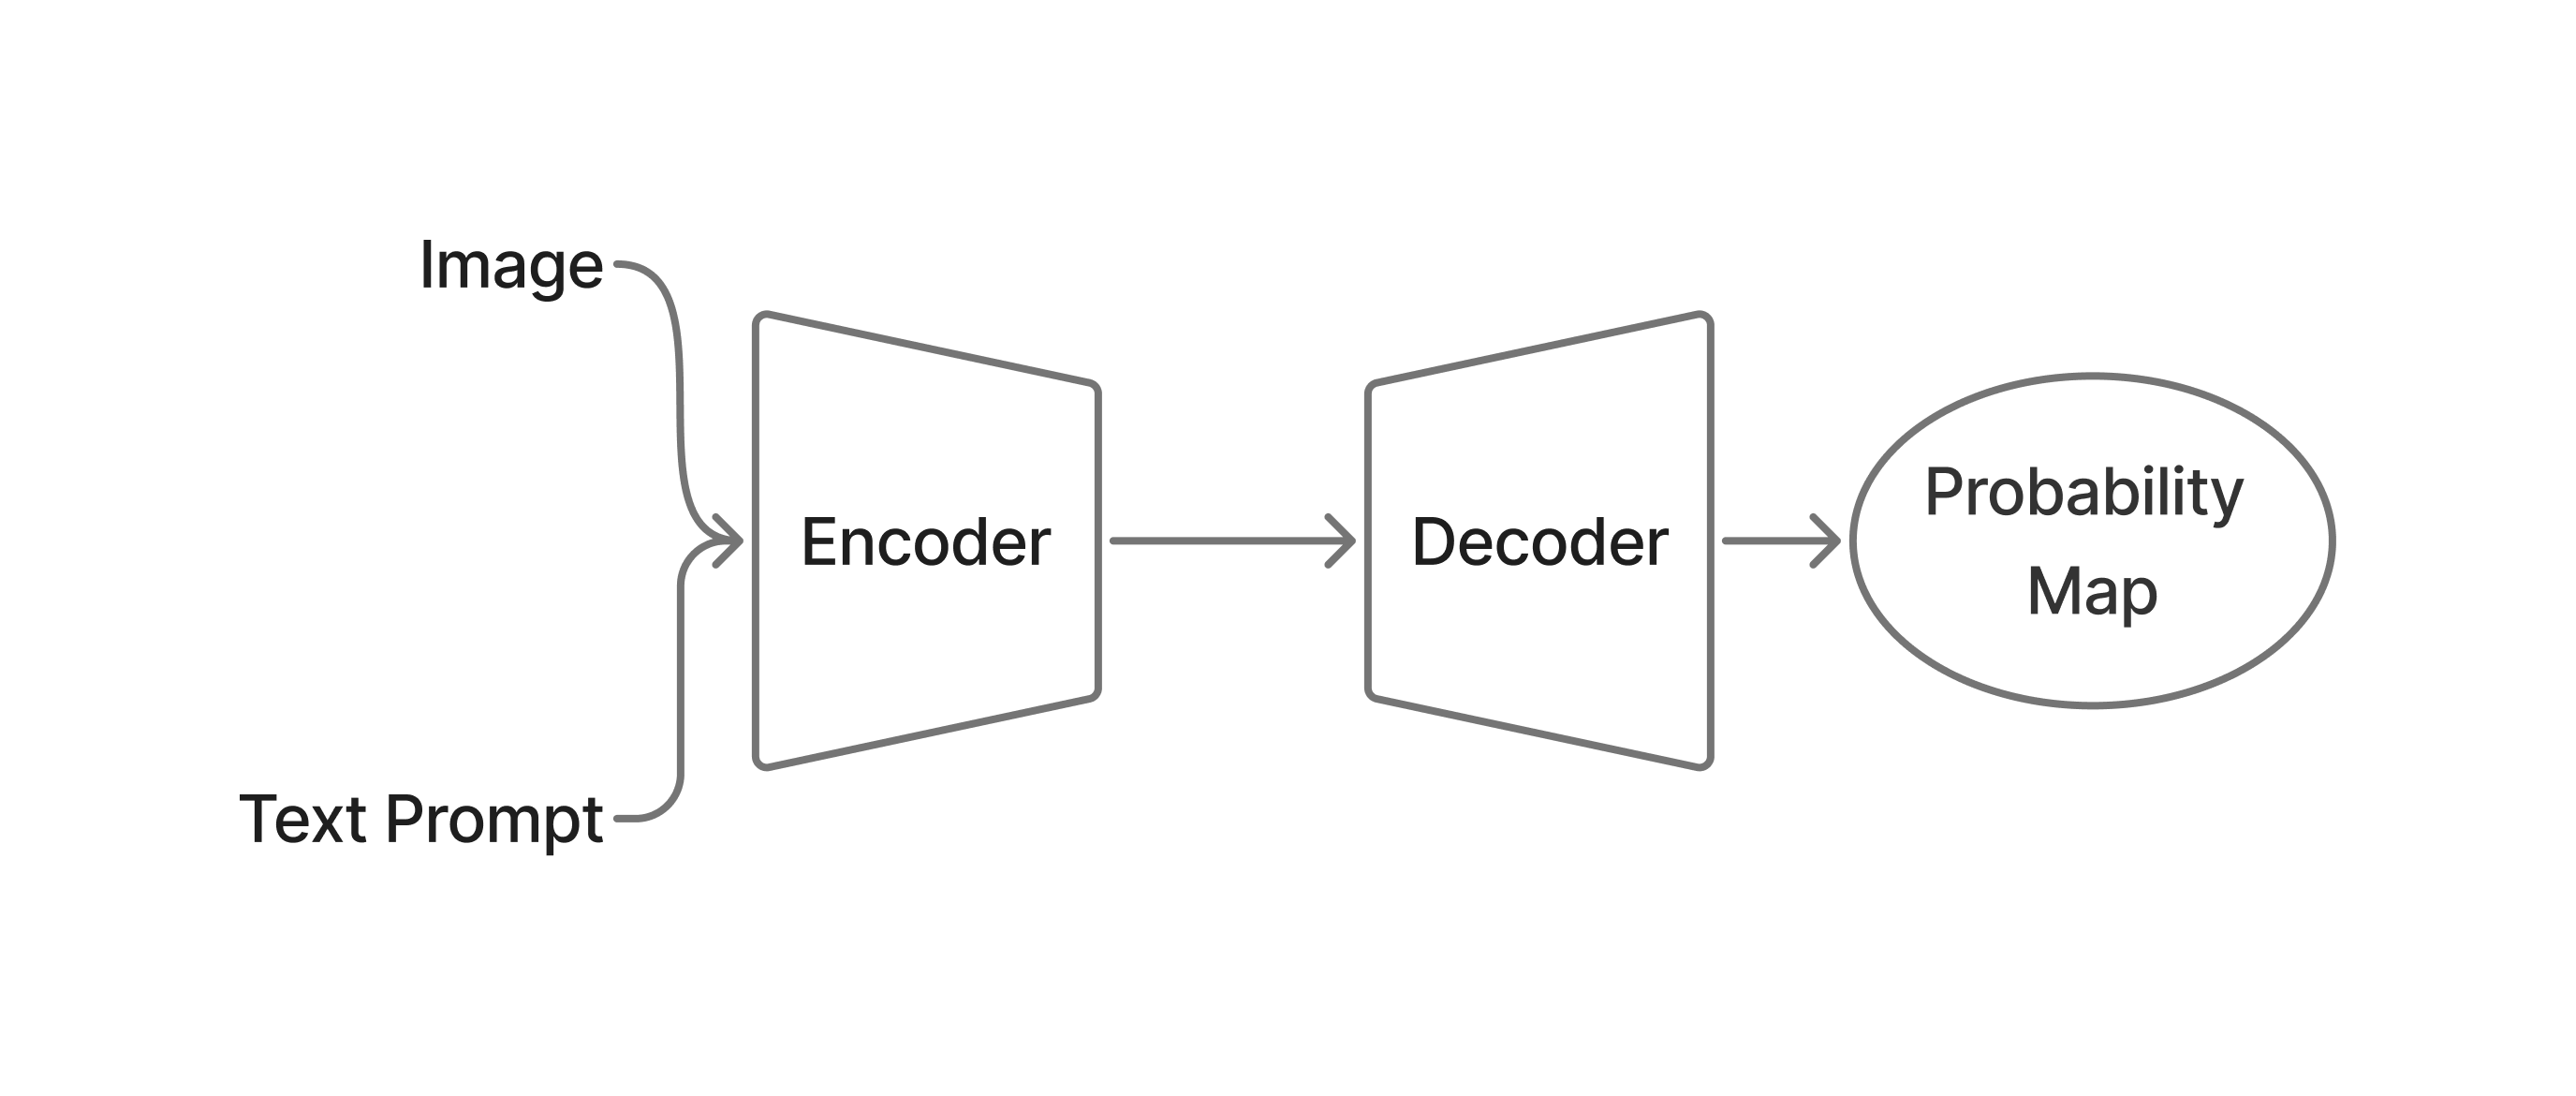
\includegraphics[width=\linewidth]{images/min-pipeline.png}
    \caption{Pipeline chung của mô hình phân đoạn dựa trên ảnh và text prompt}
\end{figure}